\documentclass[a4paper,12pt]{article}
\usepackage{geometry}
 \geometry{
 a4paper,
 total={170mm,257mm},
 left=20mm,
 top=20mm,
 }
\usepackage[export]{adjustbox} %% for picture frame
\usepackage[english]{babel}
\usepackage[utf8]{inputenc}
\usepackage{fancyhdr}
\usepackage{xcolor}

%%%question  ans enviroment 


%%% Question Environment%%%  use 
%%% Question Environment%%%  use 
%%% Question Environment%%%  use \input{./QueENV.tex}   to include
%% Use \begin{Q}....\end{Q}

\newcounter{QC}
\setcounter{QC}{1}
\newenvironment{Q}[1]{
    \section{Question -\arabic{QC}} \stepcounter{QC}{\large\textbf{#1}}
}

%%% Question Environment%%%

   to include
%% Use \begin{Q}....\end{Q}

\newcounter{QC}
\setcounter{QC}{1}
\newenvironment{Q}[1]{
    \section{Question -\arabic{QC}} \stepcounter{QC}{\large\textbf{#1}}
}

%%% Question Environment%%%

   to include
%% Use \begin{Q}....\end{Q}

\newcounter{QC}
\setcounter{QC}{1}
\newenvironment{Q}[1]{
    \section{Question -\arabic{QC}} \stepcounter{QC}{\large\textbf{#1}}
}

%%% Question Environment%%%


%%%% Anser environment use %%%% Anser environment use %%%% Anser environment use \input{./AnsENV.tex}
%% use \begin{A... {**** argument***}
\RequirePackage{scrextend}

\newenvironment{A}[1]{\textit{Answer:}{\begin{addmargin}[2em]{2em}{#1}\end{addmargin} 
  }}

% just leave some space   
%% use \begin{A... {**** argument***}
\RequirePackage{scrextend}

\newenvironment{A}[1]{\textit{Answer:}{\begin{addmargin}[2em]{2em}{#1}\end{addmargin} 
  }}

% just leave some space   
%% use \begin{A... {**** argument***}
\RequirePackage{scrextend}

\newenvironment{A}[1]{\textit{Answer:}{\begin{addmargin}[2em]{2em}{#1}\end{addmargin} 
  }}

% just leave some space   

\pagestyle{fancy}
\fancyhf{}
\rhead{\textit{Assignmnent 1}}
\lhead{\textit{074BEX403}}
\rfoot{\thepage}

\usepackage{amsmath,amssymb}

%%% format and command for lab ans c and assembly
%%%%>>>>>>>........
%%%%%% include  Titles.%%%% use \input{./CP}%%%
%%%use """"""""    \CP{}{}{}{}   """" %%%% and 4 argument to craete Title page 
%%%%%%%%%%%%%%%%%%%%%%%%%%%%%%%%%%%%%%%%%%%%%%%%%%%%%%%%%%%%%%%%%
%%%argument number
%% 1=major header ## Course name 
%% 2=minor4 heading ## lab/assignmet no
%% 3=Title  ## Assignment or Lab title
%% 4=submitted to::## input receiver Name"
%%%%%%%%%%%%%%%%%%%%%%%%%%%%%%%%%%%%%%%%%%%%%%%%%%%%%%%%%%%%%%%%%


\usepackage{mathpazo} % Palatino font
\usepackage{graphicx}
\usepackage{float}

%%% format and command for lab ans c and assembly

\newcommand{\HRule}{\rule{\linewidth}{0.4mm}} % Defines a new command for horizontal lines, change thickness here



%----------------------------------------------------------------------------------------
%	TITLE PAGE
%----------------------------------------------------------------------------------------


\newcommand{\CP}[4]{ \begin{titlepage} % Suppresses displaying the page number on the title page and the subsequent page counts as page 1
		%%%%  univerdity logo%%
		\begin{figure}[H]
			\centering
			
\includegraphics[scale=0.13]{tulogo.jpg}
		\end{figure}
		%%% end university logo

		\center % Centre everything on the page

		%------------------------------------------------
		%	Headings
		%------------------------------------------------

		\textsc{\huge Institute of Engineering \\ Central Campus,Pulchowk}\\[1.5cm] % Main heading such as the name of your university/college

		\textsc{\Large #1}\\[0.5cm] % Major heading such as course name

		\textsc{\large #2}\\[0.5cm] % Minor heading such as assignment no./ lab no.

		%------------------------------------------------
		%	Title
		%------------------------------------------------

		\HRule\\[0.4cm]

		{\Huge\bfseries #3}\\[0.4cm] % Title of your document

		\HRule\\[1.5cm]

		%------------------------------------------------
		%	Author(s)
		%------------------------------------------------
		\vfill\vfill
		\begin{minipage}{0.4\textwidth}
			\begin{flushleft}
				\large{
				\textbf{Submitted BY:}\\
				{\normalsize AMRIT PRASAD PHUYAL}\\ % NAME
				{\normalsize Roll: PULL074BEX004}} % Roll
			\end{flushleft}
		\end{minipage}
		~
		\begin{minipage}{0.4\textwidth}
			\begin{flushright}
				\large
				\textbf{Submitted To:}\\
				{ \normalsize{#4}\\ }% recepent's  Name 
				{\normalsize Department of Electronics and Computer Engineering}
			\end{flushright}
		\end{minipage}

		%------------------------------------------------
		%	Date
		%------------------------------------------------

		\vfill\vfill\vfill % Position the date 3/4 down the remaining page

		{\large\today} % Date, change the \today to a set date if you want to be precise

		\vfill % Push the date up 1/4 of the remaining page

	\end{titlepage}
}


%%% for figure 
%\begin{figure}[H]
%   \centering 
%	\includegraphics[scale=0.,cframe=blue 0.5pt 3pt]{.jpg} 
%	\textit{\caption{}}
%
%\end{figure}
%%%%
\begin{document}

%----------------------------------------------------------------------------------------
%	TITLE PAGE
%----------------------------------------------------------------------------------------
\CP{Propagation and Antenna}{Assignment \#1}
{ Propagation and Antenna}
{\textit{Dr. Ram Krishna Maharjan}\\Department of Electronics and Computer Engineering}

\pagenumbering{gobble}
\tableofcontents
\pagebreak
\listoffigures
\pagebreak
\pagenumbering{arabic}

%%%%11111111
\begin{Q}
{
    Part 1. Q.3 Different Array Antennas
}
\end{Q}

\begin{A}
    { Array antenna are the set of multiple antennas acting as the single antenna and placed closely to one another such that
     radiation pattern produced are vector sum of individual ones. These types of Array antenna increases signal strength ,
     has high directivity,gain, signal to noise ratio however it also increases resistive losses and increase external space.
    Due to these properties Array antennas are widely used in  saltellite communication, wireless communication,
    astronomical study  and in military radar too.\\

    Diferrent types of array anteena are expalined below:-

\subsection{Collinear array}
When two or more dipole antennas are vertically stacked in such a way that their corresponding elements are parallel and collinear with each other,
 it is called a collinear antenna array. 

 \begin{figure}[H]
    \centering 
	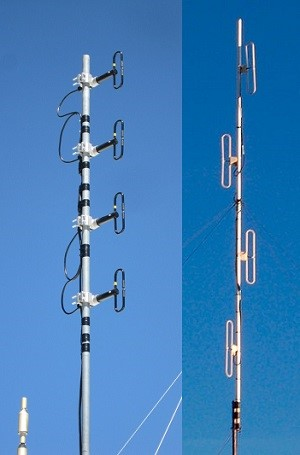
\includegraphics[scale=0.7,cframe=blue 0.5pt 3pt]{coll ant.jpg} 
	\textit{\caption{Collinear Array Antenna}}

\end{figure}

A Collinear array consists of two or more half-wave dipoles, 
which are placed end to end. These antennas are placed on a common line or axis, being parallel or collinear.
The frequency range in which the collinear array antennas operate is around 30 MHz to 3GHz which belong to the VHF and UHF bands.
These collinear arrays are uni-directional antennas having high gain. The main purpose of this array is to increase the power radiated 
and to provide high directional beam, by avoiding power loss in other directions.The antennas are mounted in such a way that every element of each antenna is in an extension of other antenna stacked upon it.
\begin{figure}[H]
    \centering 
	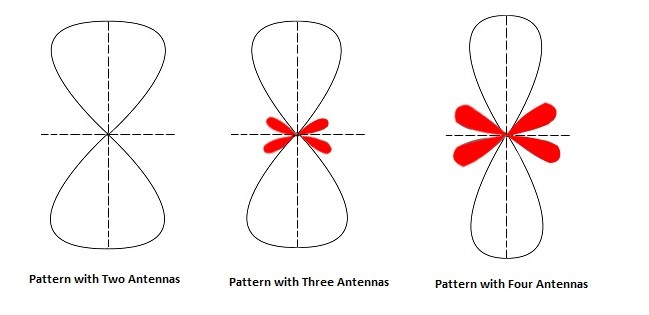
\includegraphics[scale=0.8,cframe=blue 0.5pt 3pt]{coll pat.jpg} 
	\textit{\caption{Radiation Pattern of Collinear Array Antenna}}

\end{figure}

Collinear Array antenna increases directivity,power wastage is reduced, however it can be placed outdoor only.
Due to these features it is used in UHF and VHF bands and Broadcasting purpose. 


\subsection{Broad side array}
A broadside array is a type of antenna array which is used to radiate the energy in specific direction to make better transmission. 
The broadside array is defined as the radiation pattern's direction is perpendicular or broadside to the array axis.
It uses the dipole elements that are fed in phase and separated by the one-half wave length. 
It is a bidirectional array which can send and receive process at both ends (sending and receiving end).
\begin{figure}[H]
    \centering 
	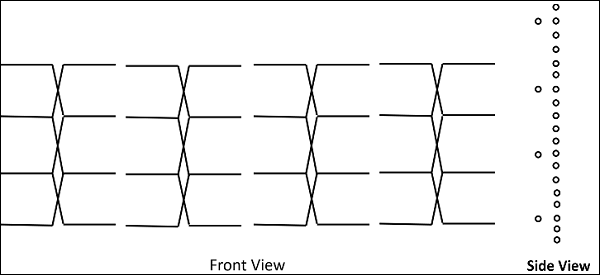
\includegraphics[scale=0.9,cframe=blue 0.5pt 3pt]{broad_side_array.jpg} 
	\textit{\caption{Front and side view Broad Size Array}}

\end{figure}


The antenna array in its simplest form, having a number of elements of equal size, equally spaced along a straight line or axis,
forming collinear points, with all dipoles in the same phase, from the same source together form the broad side array.
Typical antenna lengths in the broad side array are from 2 to 10 wavelengths. Typical spacings are \(\lambda /2  or \lambda \). 
The broad side array is strongly directional at right angles to the plane of the array. However,
 the radiation in the plane will be very less because of the cancellation in the direction joining the center.
 \begin{figure}[H]
    \centering 
	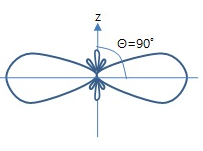
\includegraphics[scale=0.9,cframe=blue 0.5pt 3pt]{broad_side_radiation.jpg} 
	\textit{\caption{Radiation Pattern of Broad size array}}

\end{figure}
The radiation pattern of this antenna is bi-directional and right angles to the plane. The beam is very narrow with high gain.


\subsection{End fire array}
An end-fire array is an array that gives a radiation pattern whose main beam is along the axis of the array.
\begin{figure}[H]
    \centering 
	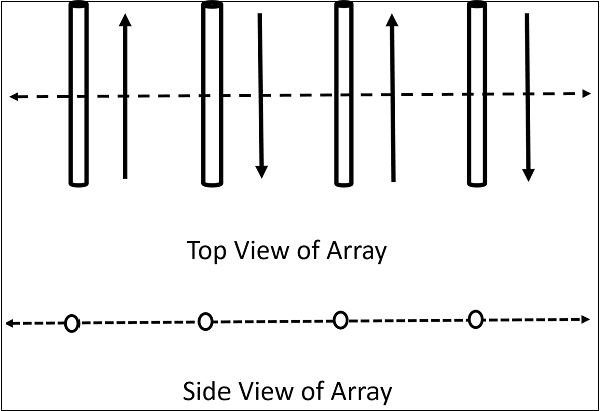
\includegraphics[scale=0.9,cframe=blue 0.5pt 3pt]{end_fire_array.jpg} 
	\textit{\caption{Top and side view from End fire array}}

\end{figure}
In a wider sense, the end-fire array is a linear or planar antenna whose direction of maximum radiation is along the line or in the plane of the array.
In End fire array, all elements are equally spaced along the array axis and fed with current of equal magnitude but their phases are different.

The radiation pattern of the broadside array is Unidirectional. A major lobe occurs at one end, where maximum radiation is present, while the minor lobes represent the losses
\begin{figure}[H]
    \centering 
	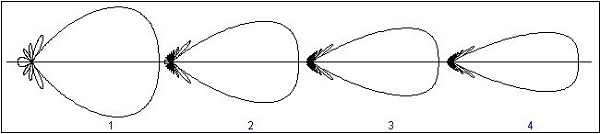
\includegraphics[scale=0.9,cframe=blue 0.5pt 3pt]{end_fire_radiation.jpg} 
	\textit{\caption{Radiation Pattern of End fire array}}

\end{figure}
Both end fire and broad side array are linear , has narrow beam and used for transmission purposes only.

\subsection{Parasitic array}
A PARASITIC ARRAY consists of one or more parasitic elements with a driven element. 
Parasitic are those which do not possess an electrical connection between them to the driven element or the feed  and
positioned so that they lie in the induction field of the driven element.The dipole that is connected to the feed is known as a driven element.
\begin{figure}[H]
    \centering 
	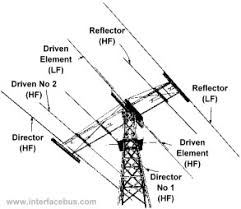
\includegraphics[scale=1.0,cframe=blue 0.5pt 3pt]{parasitic.jpg} 
	\textit{\caption{Parasitic Array}}

\end{figure}
The amount of power gain and directivity depends on the lengths of the parasitic elements and the spacing between them.
The arrays are used at frequencies ranging from 2MHz to several GHz. These are especially used to get high directivity, and better forward gain with a uni-directional.


\subsection{Yagi-Uda array}
A Yagi antenna or a Yagi-Uda antenna, is a directional antenna that radiates signals in one main direction. 
\begin{figure}[H]
    \centering 
	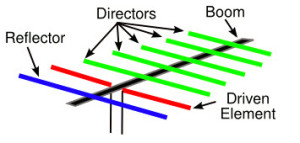
\includegraphics[scale=1.5,cframe=blue 0.5pt 3pt]{Yagi ant.jpg} 
	\textit{\caption{Yagi-Uda array Antenna}}

\end{figure}
It consists of a long transmission line with a single driven element consisting of two rods connected on either side of the transmission line. 
It also consists of a single reflector on one side of the transmission line and a number of parasitic elements which act as directors. 
The driven element of a Yagi is equivalent of a center-fed, half-wave dipole antenna. Parallel to the driven element are straight rods or wires called reflectors and directors.
A reflector is placed behind the driven element and is slightly longer than driven element; a director is placed in front of the driven element and is slightly shorter than driven element.
A typical Yagi antenna has one reflector and one or more directors.
\begin{figure}[H]
    \centering 
	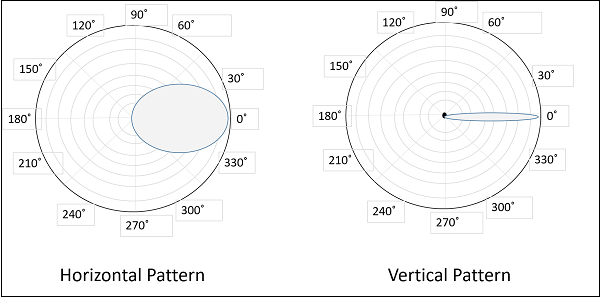
\includegraphics[scale=1.0,cframe=blue 0.5pt 3pt]{Yagi horizontal_vertical_pattern.jpg} 
	\textit{\caption{Horizontal and vertical Radiation pattern og Yagi-Uda array}}

\end{figure}
Yagi-Uda antennas has high gain,less power wastage,high directivityand covers broad range of frequencies.
 However, it is prone to noise and atmospheric effects.So , mostly use din TV reception and Single frequency application.



\subsection{Log-peroidic array}
One form of antenna that is able to provide gain and directivity along with a wide bandwidth is known as the log periodic antenna. Although larger than an equivalent Yagi or other directive design for an equivalent level of gain, 
it provides the capability to operate on many different frequencies.
\begin{figure}[H]
    \centering 
	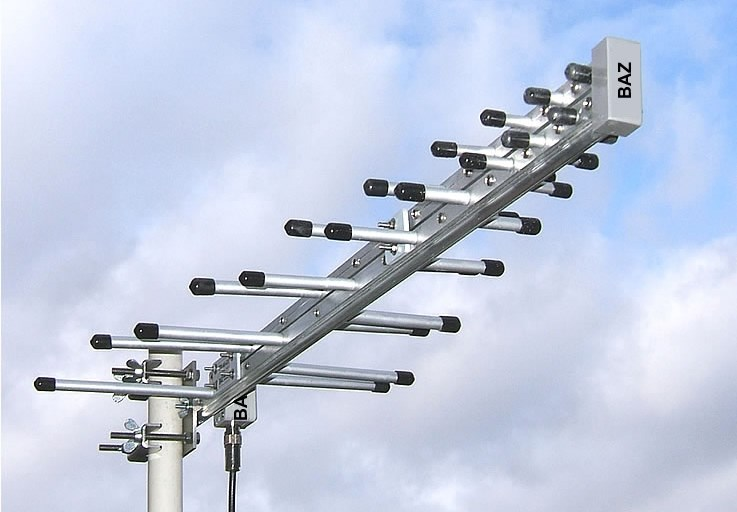
\includegraphics[scale=0.6,cframe=blue 0.5pt 3pt]{Log-Antenna.jpg} 
	\textit{\caption{Log-periodic Antenna}}

\end{figure}
A log-periodic antenna is a group of dipole antennas of varying sizes strung together and fed alternately through a common transmission line. 
The dipole antennas diminish in size from the back to the front. The element at the back of the array which is the largest, 
acts as a half wave dipole at the lowest frequency and that at the front is a half wavelength at the highest frequency of operation. 
This unique configuration, enables Log-periodic antennas to have wide bandwidths.
The frequency range, in which the log-periodic antennas operate is around 30 MHz to 3GHz which belong to the VHF and UHF bands.
There are several type of log-periodic antennas such as the planar, trapezoidal, zig-zag, V-type, slot and the dipole.
\begin{figure}[H]
    \centering 
	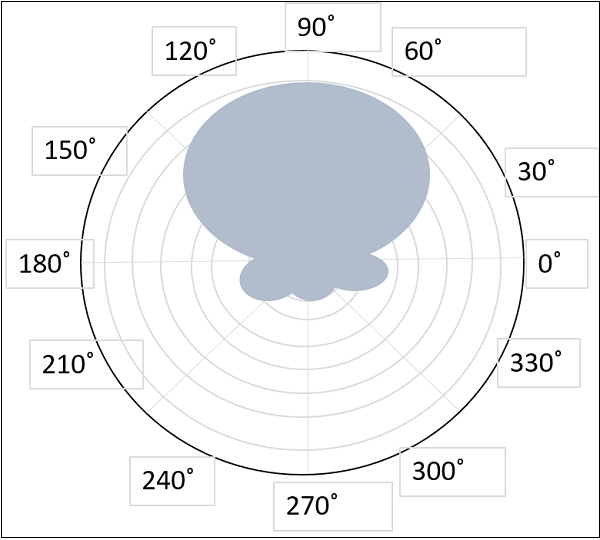
\includegraphics[scale=0.8,cframe=blue 0.5pt 3pt]{log_periodic radiation.jpg} 
	\textit{\caption{Radiation pattern of Log- periodic antenna}}

\end{figure}
Log-periodic has compact design and the gain and radiation pattern can be tuned as per requirement. The installtion cost is high and it has to be external mount.
It is used in HF communication and particular Tv reception and aslo use dfor all round monitoring in higher frequency bands.
    }
\end{A}

%%%%%%%%%%%

%%%%%%%2222222222

\begin{Q}
    {
        Part 2. Q.3 List out the major parameters of the antenna. Define four of them with mathematical expression if necessary.
        Sketch symmetrical gregorian type antenna.
    }
\end{Q}

\begin{A}
    {
        Some of the major parameters of anteena are defiend below:-


\subsection{Directivity}
The ratio of maximum radiation intensity of the subject antenna to the radiation intensity of an isotropic or reference antenna, 
radiating the same total power is called the directivity.
Directivity is a dimensionless ratio and may be expressed numerically or in decibels (dB).
Its radiation intensity is focused in a particular direction, while it is transmitting or receiving. 
Hence, the antenna is said to have its directivity in that particular direction.
If that particular direction is not specified, then the direction in which maximum intensity is observed,
 can be taken as the directivity of that antenna.
 The directivity of a non-isotropic antenna is equal to the ratio of the radiation intensity in a given direction to the radiation intensity of the isotropic source.\\
 
 \textbf{Mathematically,}

    \begin{align*}
Directivity &=  \frac{Maximum radiation intensity of subject antenna}{Radiation intensity of an isotropic antenna}\\
D &=  \frac{\phi(\theta,\phi)_{max}(from  subject antenna)} {\phi_{0}(from  an isotropic antenna) }\\
    \end{align*}

Where,\\

\({\phi(\theta,\phi)_{max}}\) is the  maximum radiation intensity of subject antenna.\\

\({\phi_{0}}\)  is the radiation intensity of an isotropic antenna (antenna with zero losses).




\subsection{Aperture efficiency}
Aperture efficiency of an antenna, is the ratio of the effective radiating area (or effective area) to the physical area of the aperture.
An antenna has an aperture through which the power is radiated. This radiation should be effective with minimum losses. 
The physical area of the aperture should also be taken into consideration,
 as the effectiveness of the radiation depends upon the area of the aperture, physically on the antenna.\\

 \textbf{Mathematically,}
    \begin{align*}
        \varepsilon_{A} = \frac{A_{eff}}{A_{p}}
    \end{align*}  

    Where,\\

     \(\varepsilon_{A}\) is Aperture Efficiency.\\

     \({A_{eff}}\) is effective area.\\

     \({A_{p}}\)  is physical area.\\


\subsection{Antenna Efficiency}
Antenna Efficiency is the ratio of the radiated power of the antenna to the input power accepted by the antenna
Simply, an Antenna is meant to radiate power given at its input, with minimum losses. 
The efficiency of an antenna explains how much an antenna is able to deliver 
its output effectively with minimum losses in the transmission line.
This is otherwise called as Radiation Efficiency Factor of the antenna.\\

\textbf{Mathematically,}
\begin{align*}
    \eta_{e} = \frac{P_{rad}}{P_{input}}
\end{align*}

Where,\\

\(\eta_{e}\) is the antenna efficiency.\\

\({P_{rad}} \) is the antenna efficiency.\\

\({P_{input}}\) is the input power for the antenna.\\

\subsection{Gain}
Gain of an antenna is the ratio of the radiation intensity in a given direction to the
 radiation intensity that would be obtained if the power accepted by the antenna were radiated isotropically.
 Simply, gain of an antenna takes the directivity of antenna into account along with its effective performance.
  If the power accepted by the antenna was radiated isotropically (that means in all directions),
  then the radiation intensity we get can be taken as a referential. 
  It describe how much power is transmitted in the direction of peak radiation to that of an isotropic source.
  Its unit is \textbf{dB}\\

\textbf{Mathematically,}
\begin{align*}
    G = \eta_{e}D
\end{align*}

Where,\\

\(G\) is the antenna efficiency.\\

\(\eta_{e} \) is the antenna efficiency.\\

\(D\) is the input power for the antenna.\\


\begin{figure}[H]
    \centering 
	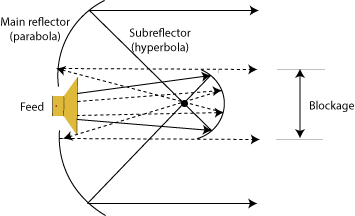
\includegraphics[scale=0.856,cframe=blue 0.5pt 3pt]{gregorian_architecture.png} 
	\textit{\caption{Gregorian Type Antenna with Concave reflector}}

\end{figure}

}
\end{A}

\end{document}